\documentclass[9pt, aspectratio=169]{beamer}
\usepackage{FiraSans}
\usetheme{metropolis}
\usepackage[utf8]{inputenc}
\usepackage{amsmath}
\usepackage{amsfonts}
\usepackage{amssymb}
\usepackage{multicol}
\usepackage{tikz}
\usepackage{xcolor}
\usepackage[T1]{fontenc} 
\usepackage[skins]{tcolorbox}
\author{Nicola Roman\`o - nicola.romano@ed.ac.uk}
\title{Basic image manipulation in Python}
\setlength{\fboxsep}{0pt}
\setbeamertemplate{caption}{\raggedright\insertcaption\par}
\setbeamertemplate {footline}{\begin{scriptsize}\hfill\insertframenumber ~of \inserttotalframenumber\kern1em\vskip5pt\end{scriptsize}}

%\setbeamercovered{transparent} 
%\setbeamertemplate{navigation symbols}{} 

\titlegraphic{\centering \includegraphics[scale=.5]{instituteLogo.png}}
\date{}

\AtBeginSection[]
{
  \begin{frame}<beamer>
    {Outline}
    \huge{\tableofcontents[currentsection, currentsubsection]}
  \end{frame}
}

\AtBeginSubsection[]
    {
    \begin{frame}<beamer>
        {Outline}
        \huge{\tableofcontents[currentsection, currentsubsection]}
        \end{frame}        
    }

\begin{document}

\newtcolorbox{codebox}{enhanced,
    top=2pt,
    left=2pt,
    right=2pt,
    bottom=2pt,
    boxrule=0pt,
    leftrule=5pt,
    sharp corners,
    colback=gray!20,
    colframe=blue!60!black}

\begin{frame}
    \titlepage
\end{frame}

\begin{frame}
    {Learning objectives}
    \begin{columns}
        \begin{column}{0.8\textwidth}
            \begin{itemize}
                \item Perform basic image manipulation (cropping, scaling, rotating, etc)
                \item Interpret and manipulate image histograms
            \end{itemize}
        \end{column}
        \begin{column}{0.2\textwidth}
            
\includegraphics[angle=-30, origin=tr, width=1.5\textwidth]{lightbulb.png}
        \end{column}
    \end{columns}
\end{frame}

\section{A brief recap}

\begin{frame}
    {Python tools for image processing}
    \centering
    Last time we learnt how to open and display images using Python.

    \vspace{3em}

    \begin{columns}
        \begin{column}{0.3\textwidth}
            \includegraphics[width=0.8\textwidth]{matplotlib_logo.png}
            General plotting library
        \end{column}
        \begin{column}{0.3\textwidth}
            \includegraphics[width=0.8\textwidth]{skimage_logo.png}
            Specific functions for image manipulation
        \end{column}
        \begin{column}{0.3\textwidth}
            \includegraphics[width=0.8\textwidth]{numpylogo.png}
            Library for matrix operations
        \end{column}
    \end{columns}
\end{frame}

\begin{frame}
    {Reading images as Numpy arrays}
    \begin{columns}
        \begin{column}{0.5\textwidth}
            \begin{center}
                \includegraphics[width=0.5\textwidth]{matplotlib_logo.png}
            \end{center}
            \begin{codebox}
                \texttt{import matplotlib.pyplot as plt\\
                    img = plt.imread("cells.jpg")\\
                    plt.imshow(img)\\
                    plt.show()
                }
            \end{codebox}
        \end{column}
        \begin{column}{0.5\textwidth}
            \begin{center}
                \includegraphics[width=0.5\textwidth]{skimage_logo.png}
            \end{center}
            \begin{codebox}
                \texttt{from skimage import io\\
                    img = io.imread("cells.jpg")\\
                    io.imshow(img)\\
                    io.show()
                }
            \end{codebox}
        \end{column}
    \end{columns}
\end{frame}

\begin{frame}
    {Colour mapping}
    \begin{columns}
        \begin{column}{0.6\textwidth}
            \begin{codebox}
                \texttt{fig, ax = plt.subplots(ncols=2, nrows=2)\\
                    ax[0, 0].imshow(img, "gray")\\
                    ax[0, 1].imshow(img, "viridis")\\
                    ax[1, 0].imshow(img, "Greens")\\
                    ax[1, 1].imshow(img, "PuBu")}
            \end{codebox}
        \end{column}
        \begin{column}{0.4\textwidth}
            \includegraphics[width=\textwidth]{nuclei_cmapped.png}
        \end{column}
    \end{columns}
    \centering

    Check out the Matplotlib website for a list of colourmaps! \url{https://matplotlib.org/stable/tutorials/colors/colormaps.html}

\end{frame}

\section{Basic image operations}

\begin{frame}
    {Basic image operations}
    Often you will need to crop, scale or rotate an image before further manipulation.
    There are many use cases for this, including

    \begin{itemize}
        \item Analysing only part of an image (cropping)
        \item Making sure all input images for a pipeline are the same size (scaling, cropping)
        \item Aligning multiple images (e.g. in video stabilization) (rotating)
        \item \dots
    \end{itemize}
    \centering
    
\includegraphics[width=0.4\textwidth]{basic_manipulation.png}
\end{frame}

\subsection{Cropping}

\begin {frame}
{Cropping}
Cropping is as easy as subsetting the image matrix.

\begin{codebox}
    \texttt{\# Assume we loaded a 512 x 512 image in the img variable\\
        \# Take the top-left 100 x 100 pixels\\
        img1 = img[0:100, 0:100] \# shape (100, 100)\\
        \pause
        \# Take a 100 pixel wide strip on the left of the image\dots\\
        img2 = img[:, 0:100] \# shape (512, 100)\\
        \# Or on the right!\\
        img3 = img[:, -100:] \# shape (512, 100)
    }
\end{codebox}
\end{frame}

\begin{frame}
    {Cropping in more than two dimensions}
    Since images are just tensors, we can crop them in any dimensions.
    \begin{codebox}
        \texttt{\# We loaded a 512 x 512 RGB image in img\\
            \# img.shape is (3, 512, 512)\\
            \# Extract the green channel\\
            img\_green = img[1] \# Shape (512, 512)\\
            \pause
            $~$\\
            \# We have a 512 x 512 video of 300 frames\\
            \# Take the first 50 frames\\
            \# video.shape is (300, 512, 512)\\
            video\_crop = video[0:50]
        }
    \end{codebox}
\end{frame}

\begin{frame}
    {Question time}
    \begin{columns}
        \begin{column}{0.7\textwidth}
            We have a 100 frames video of a 512 x 512 z-stack with 60 planes loaded in \texttt{zstack}.\\
            \texttt{zstack.shape} is \texttt{(100, 60, 512, 512)}\\
            \vspace*{2em}
            \centering
            \textbf{What does this code give you?}
            \vspace{2em}
            \begin{codebox}
                \texttt{result = stack[50:70, :, 100:300]}
            \end{codebox}
        \end{column}
        \begin{column}{0.3\textwidth}
            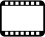
\includegraphics[width=.7\textwidth]{video.png}
        \end{column}
    \end{columns}
\end{frame}

\subsection{Scaling}

\begin{frame}
    {Scaling}
    \centering
    
\includegraphics[width=.3\textwidth]{scaling.png}\\
    Two problems:\\
    When \textbf{upscaling} we need to generate new information.
    \\
    When \textbf{downscaling} we need to decide "how to lose" information.
\end{frame}

\begin{frame}
    {Nearest-neighbor interpolation}
    The simplest way to resize an image is to use nearest neighbor interpolation. Each pixel of the scaled image will have the colour of the nearest pixel in the original image.\\

    In this "1D" example, we resize a 1x2 image to 1x6

    \centering
    \includegraphics[width = 0.4\textwidth]{1D_NN_interpolation.png}
\end{frame}

\begin{frame}
    {Nearest-neighbour interpolation}
    \begin{figure}
        \centering
        \includegraphics[width=.65\textwidth]{upscaling_no_interpolation.png}
        \caption{Upscaling of a 5x5 image by a factor of 2, to get a 10x10 image, with nearest neighbour interpolation}
    \end{figure}
    \pause
    \begin{codebox}
        \texttt{from skimage.transform import rescale\\
            img\_scaled = rescale(img, 2, order=0)}
    \end{codebox}
\end{frame}

\begin{frame}
    {Scaling with interpolation}
    Better ways to scale an image involve changing the pixel values of the rescaled image based on their neighbourhood.\\
    For example we could use linear interpolation
    \centering
    \includegraphics[width=0.65\textwidth]{1D_lin_interpolation.png}
\end{frame}

\begin{frame}
    {Linear interpolation}
    The same applies in 2D, although we need to take into accounts the values of both horizontal and vertical neighbours (bilinear interpolation).
    \begin{figure}
        \centering
        \includegraphics[width=.65\textwidth]{upscaling_lin_interpolation.png}
        \caption{Upscaling of a 5x5 image by a factor of 2, to get a 10x10 image, with bi-linear interpolation}
    \end{figure}

    \begin{codebox}
        \texttt{from skimage.transform import rescale\\
            img\_scaled = rescale(img, 2, order=1)}
    \end{codebox}
\end{frame}

\begin{frame}
    {Nearest neighbor vs linear interpolation}
    \begin{figure}

        \centering
        \includegraphics[width=0.4\textwidth]{interpolation schematics.png}
        \caption{Comparison of nearest neighbour and linear interpolation - Source: \href{https://en.wikipedia.org/wiki/Nearest-neighbor_interpolation}{Wikipedia}}
    \end{figure}
\end{frame}

\begin{frame}
    {Higher orders of interpolation}
    We can use higher orders of interpolation to produce smoother results. \\
    \begin{figure}

        \centering
        \includegraphics[width=0.55\textwidth]{interpolations.png}
        \caption{Comparison of nearest neighbour and linear interpolation - Source: \href{https://en.wikipedia.org/wiki/Nearest-neighbor_interpolation}{Wikipedia}}
    \end{figure}

    Scikit Image supports values from 0 to 5 in the \texttt{order} parameter of the \texttt{rescale} function. 0 is nearest neighbor, 1 is bi-linear, 2 is bi-quadratic and so on.
\end{frame}

\begin{frame}
    {Scaling to a target size}
    To scale to a target size, rather than by a specific factor, we can use \texttt{resize} instead of \texttt{rescale}.

    \begin{codebox}
        \texttt{import matplotlib.pyplot as plt\\
            from skimage.transform import resize, rescale\\
            \\
            img = plt.imread("cells.jpg")\\
            img\_scaled1 = rescale(img, 2)\\
            img\_scaled2 = resize(img, (150, 150))
        }
    \end{codebox}
\end{frame}

\begin{frame}
    {Local mean downscaling}
    Another simple solution for downscaling is calculating the local mean of each pixel
    \centering
    \includegraphics[width=.65\textwidth]{downscale.png}
    \pause
    \begin{codebox}
        \texttt{from skimage.transform import downscale\_local\_mean\\
            img\_small = downscale\_local\_mean(img, (2,2))}
    \end{codebox}

    Image needs to be padded if the size is not a multiple of the downscaling factor. This method is fast but not good at keeping fine details.
\end{frame}

\begin{frame}
    {Scaling summary}
    \texttt{skimage.transform.rescale} $\rightarrow$ scales an image by a specific factor (>1 upscaling; <1 downscaling.). Can specify a different scaling factor for each dimension of the image.
    \vspace{2em}

    \texttt{skimage.transform.resize} $\rightarrow$ scales an image to a target size.
    \vspace{2em}

    \texttt{skimage.transform.downscale\_local\_mean} $\rightarrow$ downscales the image by a specific factor (>1), using the local mean of each pixel.
\end{frame}

\subsection{Rotating}

\begin{frame}
    {Rotating a point around the origin}
    \centering
    We want to rotate a point $P (x,y)$ around the origin by an angle $\theta$ to get $P' (x',y')$.\\
    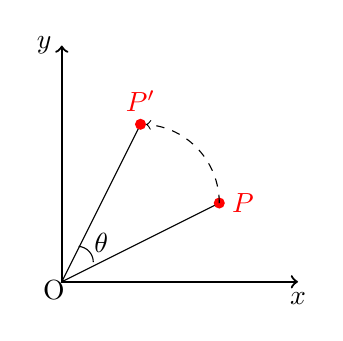
\begin{tikzpicture}
        \draw [<->,thick] (0,3) node (yaxis) [left] {$y$}
        |- (3,0) node (xaxis) [below] {$x$};
        \draw [thin] (1,2) -- (0,0) -- (2,1);
        \fill[red] (1, 2) circle (2pt) node at (1, 2.3) {$P'$};
        \fill[red] (2, 1) circle (2pt) node at (2.3, 1) {$P$};
        \draw [->, dashed] (2,1) arc (0:86:1);
        \draw (.4,.25) arc (0:86:.2) node at (.5, .5) {$\theta$};
        \node at (-.1, -.1) {O};
    \end{tikzpicture}
\end{frame}

\begin{frame}
    {Rotating a point around the origin}
    \center
    {
        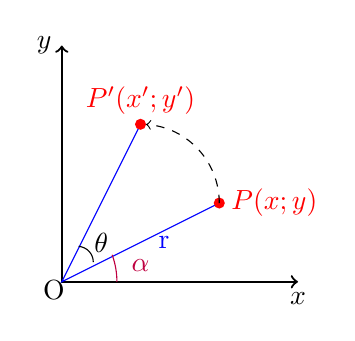
\begin{tikzpicture}
            % Axes
            \draw [<->,thick] (0,3) node (yaxis) [left] {$y$}
            |- (3,0) node (xaxis) [below] {$x$};
            \draw [thin, blue] (1,2) -- (0,0) -- (2,1);
            % Points
            \fill[red] (1, 2) circle (2pt) node at (1, 2.3) {$P' (x'; y')$};
            \fill[red] (2, 1) circle (2pt) node at (2.7, 1) {$P (x; y)$};
            % Rotation arrow
            \draw [->, dashed] (2,1) arc (0:86:1);
            % Angle theta
            \draw (.4,.25) arc (0:86:.2) node at (.5, .5) {$\theta$};
            % Angle alpha
            \draw [purple] (.7,0) arc (0:20:1) node at (1, .2) {$\alpha$};
            % Origin
            \node at (-.1, -.1) {O};
            % Radius
            \node [blue] at (1.3, .5) {r};
        \end{tikzpicture}
    }

    \begin{columns}
        \begin{column}{0.5\textwidth}
            $$P: \begin{cases}x = r~\text{cos}(\alpha)\\y = r~\text{sin}(\alpha)\end{cases}
                P': \begin{cases}x' = r~\text{cos}(\alpha+\theta)\\y' = r~\text{sin}(\alpha+\theta)\end{cases}$$
        \end{column}
        \pause
        \begin{column}{0.5\textwidth}
            \centering
            $$P': \begin{cases}x' = r~\text{cos}(\alpha)\text{cos}(\theta)-r~\text{sin}(\alpha)\text{sin}(\theta)\\y' = r~\text{sin}(\alpha)\text{cos}(\theta)+r~\text{sin}(\theta)\text{cos}(\alpha)\end{cases}$$

            Why? \href{https://en.wikipedia.org/wiki/List\_of\_trigonometric\_identities\#Angle\_sum\_and\_difference\_identities}{\underline{Wikipedia to the rescue!}}
        \end{column}
    \end{columns}
    \pause
    Thus:
    \begin{columns}
        \begin{column}{0.5\textwidth}
            $$P': \begin{cases}x' = x~\text{cos}(\theta)-y~\text{sin}(\theta)\\y' = y~\text{cos}(\theta)+x~{sin}(\theta)\end{cases}$$
        \end{column}
        \pause
        \begin{column}{0.5\textwidth}
            $$\begin{bmatrix}x'\\y'\end{bmatrix} = \color{red}\begin{bmatrix}\text{cos}\theta&-\text{sin}\theta\\\text{sin}\theta&\text{cos}\theta\end{bmatrix}\color{black}\begin{bmatrix}x\\y\end{bmatrix}$$
            \centering
            \color{red}Transformation (rotation) matrix
        \end{column}
    \end{columns}
\end{frame}

\begin{frame}
    {Rotating in Scikit Image}
    To rotate an image we will:
    \begin{itemize}
        \item Offset our image so that it is centered on the origin
        \item Generate a rotation matrix
        \item Multiply the coordinates of each pixel by the rotation matrix
    \end{itemize}
    \pause
    Luckily, Scikit Image has a ready function for that, \texttt{skimage.transform.rotate}.

    \begin{columns}
        \begin{column}{0.5\textwidth}
            \begin{codebox}
                \texttt{import matplotlib.pyplot as plt\\
                    from skimage.transform import rotate\\
                    \\
                    img = plt.imread("cells.jpg")\\
                    img\_rotated = rotate(img, 20)\\
                    \\
                    plt.imshow(img\_rotated, cmap="gray")\\
                    plt.show()}
            \end{codebox}
        \end{column}
        \begin{column}{0.5\textwidth}
            \begin{figure}
            \includegraphics[width=\textwidth]{rotate_image.png}
            \caption{Note: we lost part of the image and we "gained" black pixels around it. By default, \texttt{rotate} performs bilinear interpolation.}
            \end{figure}
        \end{column}
    \end{columns}
\end{frame}

\begin{frame}
    {Optional exercise - want to try by yourself?}
    It might be interesting to try to code image rotation by yourself.

    Hints:

    \begin{itemize}
        \item You can generate transformation matrices using \texttt{skimage.transform.SimilarityTransform}
        \item You will need three matrices: one translation matrix to offset your image by (-xcenter, -ycenter); a rotation matrix to rotate your image; and finally another translation matrix to translate your image back to its original position.
        \item You can combine the matrices as \texttt{m1+m2+m3}
        \item You can use \texttt{skimage.transform.warp} to apply the transformation matrix to your image.
    \end{itemize}

    If you are stuck, try to look at the \href{https://github.com/scikit-image/scikit-image/blob/main/skimage/transform/\_warps.py\#L349-L460}{\underline{source code for rotate}}!
\end{frame}
\end{document}

